\subsection*{Results}
\subsubsection*{Average End-to-end distance $R$}

In Figure \ref{fig:etoe} the square of the average End-to-end distance $R^2$ as a function of length $N$ is seen.

\begin{figure}[htb]
        \centering
        \begin{subfigure}[b]{0.45\textwidth}
                \centering
                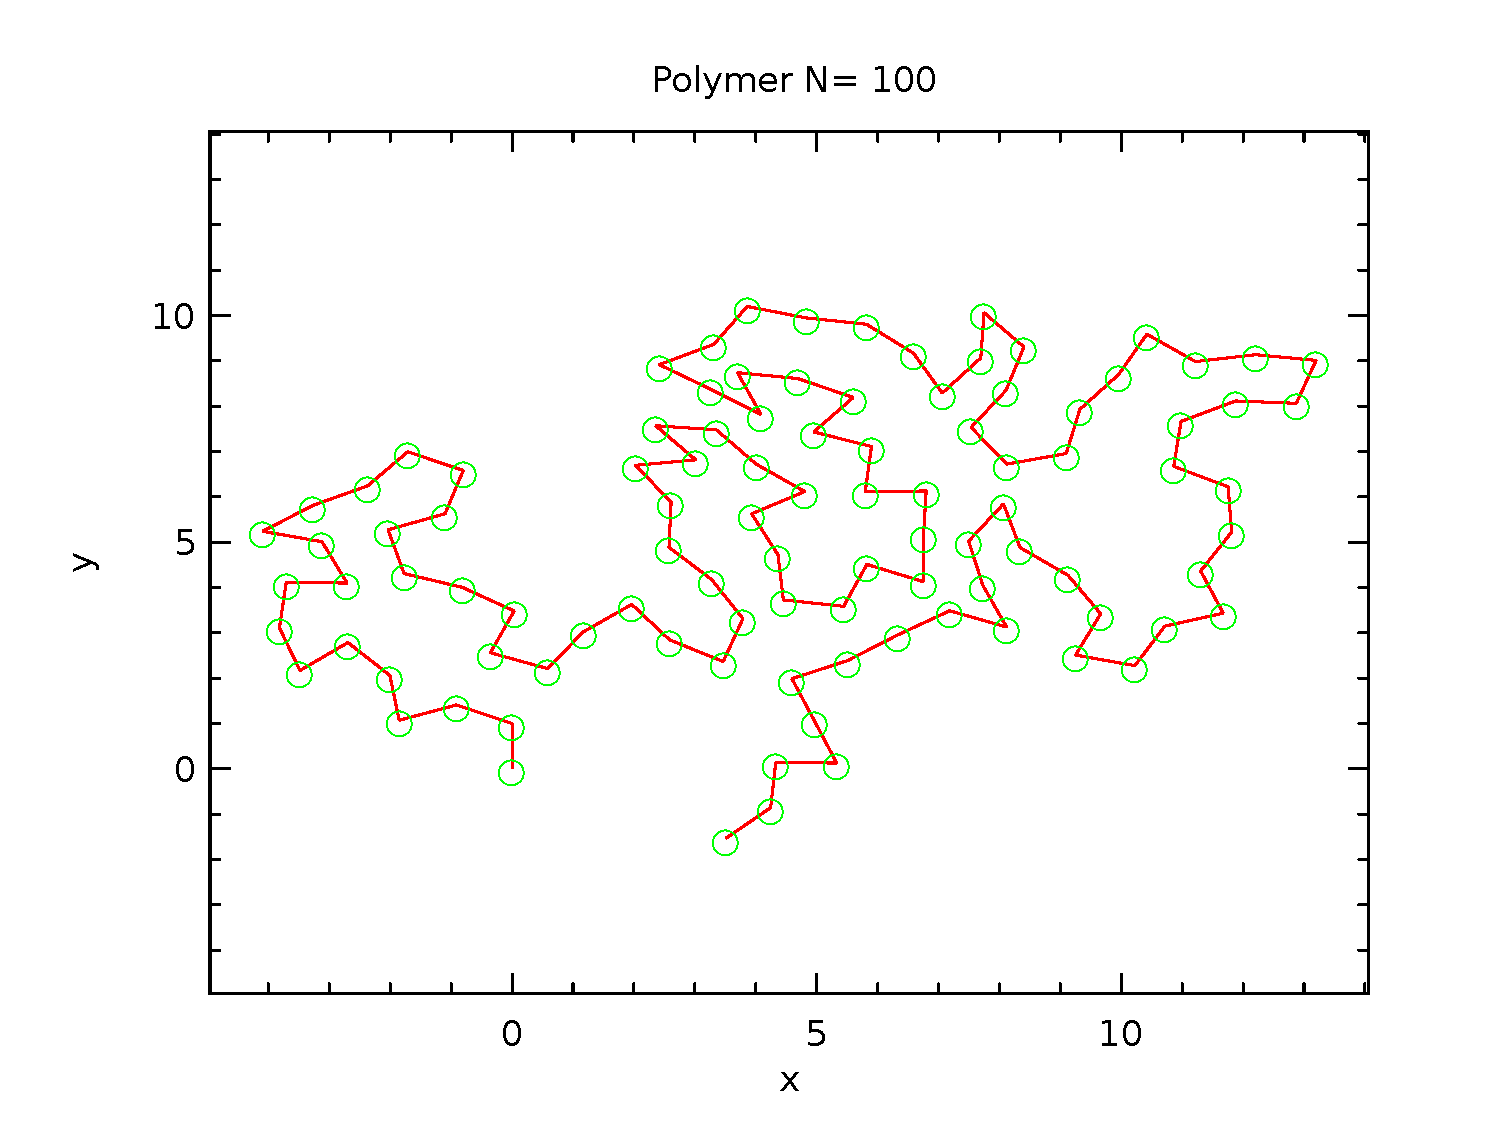
\includegraphics[width=\textwidth]{voorblad.pdf}
                \caption{Without Pruning and Enrichment, $a= ...$.}
                \label{fig:etoe_noprem}
        \end{subfigure}
	\quad
        \begin{subfigure}[b]{0.45\textwidth}
                \centering
                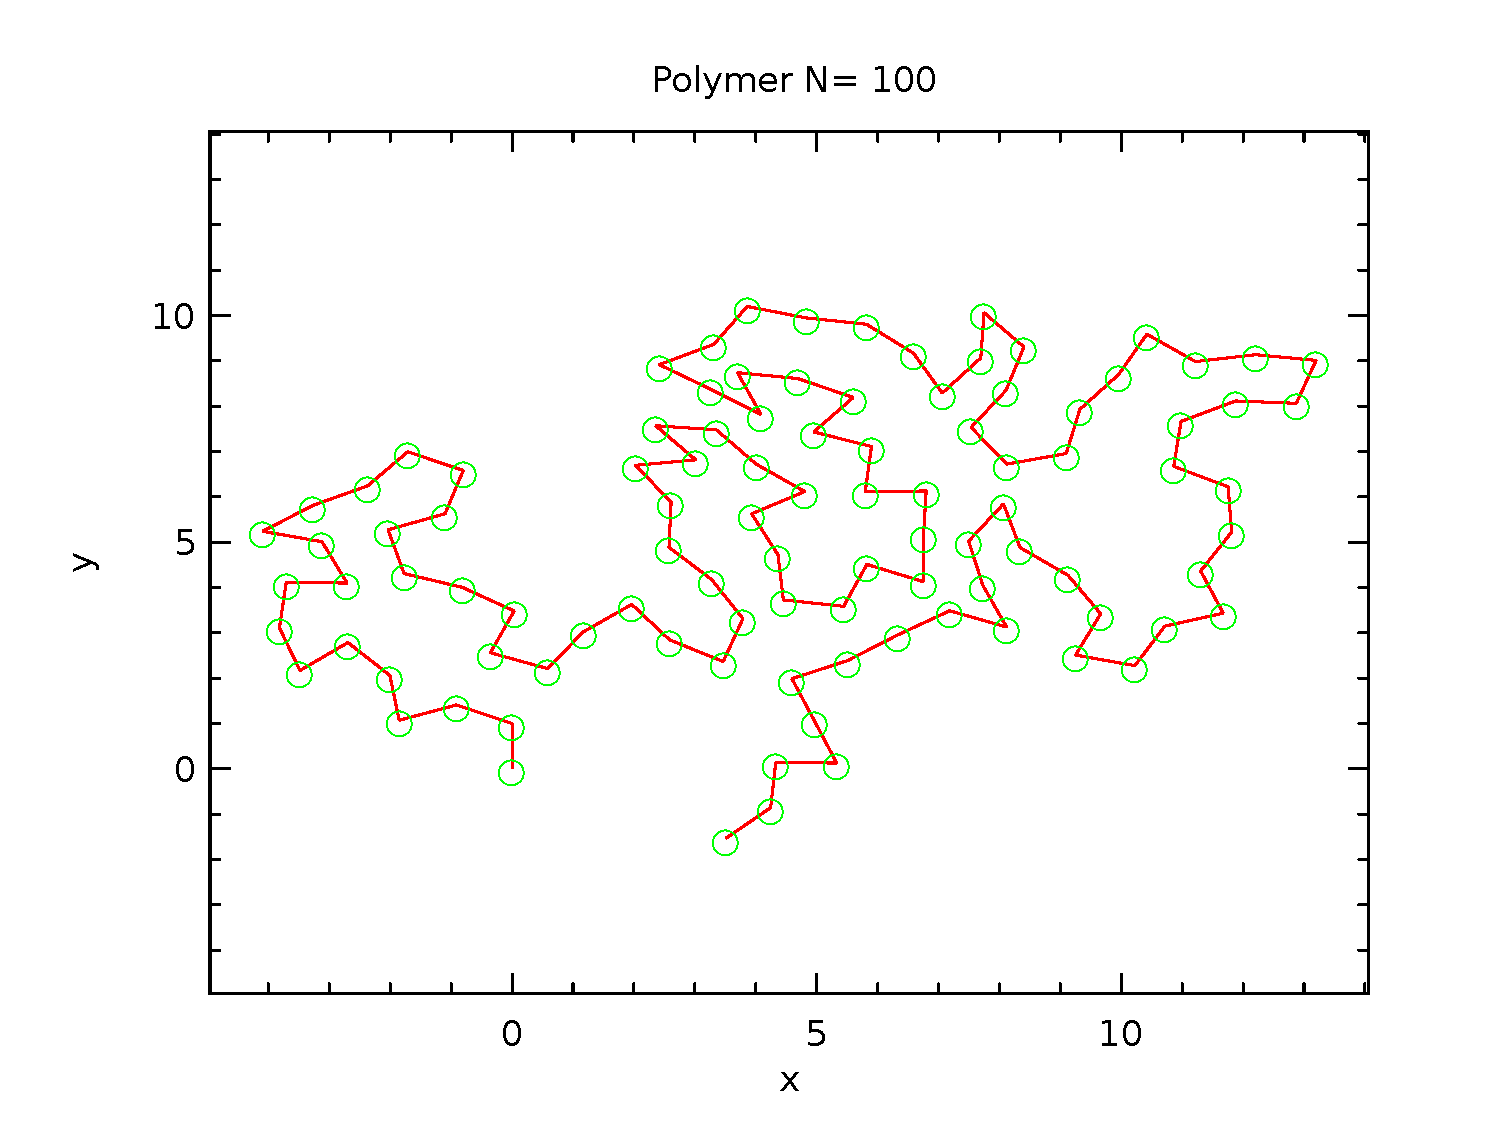
\includegraphics[width=\textwidth]{voorblad.pdf}
                \caption{With Pruning and Enrichment, $a= ...$.}
                \label{fig:etoe_prem}
        \end{subfigure}
        \caption{Square of the End-to-end distance $R^2$ as a function of polymer length $N$, the red dotted line is the theoretical fit of $R^2=a\cdot N^{3/2}$ to the data, the population sizes for each length $N$ are given as well.}
        \label{fig:etoe}
\end{figure}

It is seen that the results for $N>100$ are a lot better if PERM is being implemented. This is expected because the longer the polymer becomes the higher the probability that it traps itself. If PERM is being implemented a polymer can't go on after trapping itself and the values are $R^2$ agree with the theoretical value again. 


\subsubsection*{Average Gyradius $G$}

In Figure \ref{fig:gyradius} the average Gyaradius $G$ as a function of length $N$ is seen.


\begin{figure}[ht!]
\centering
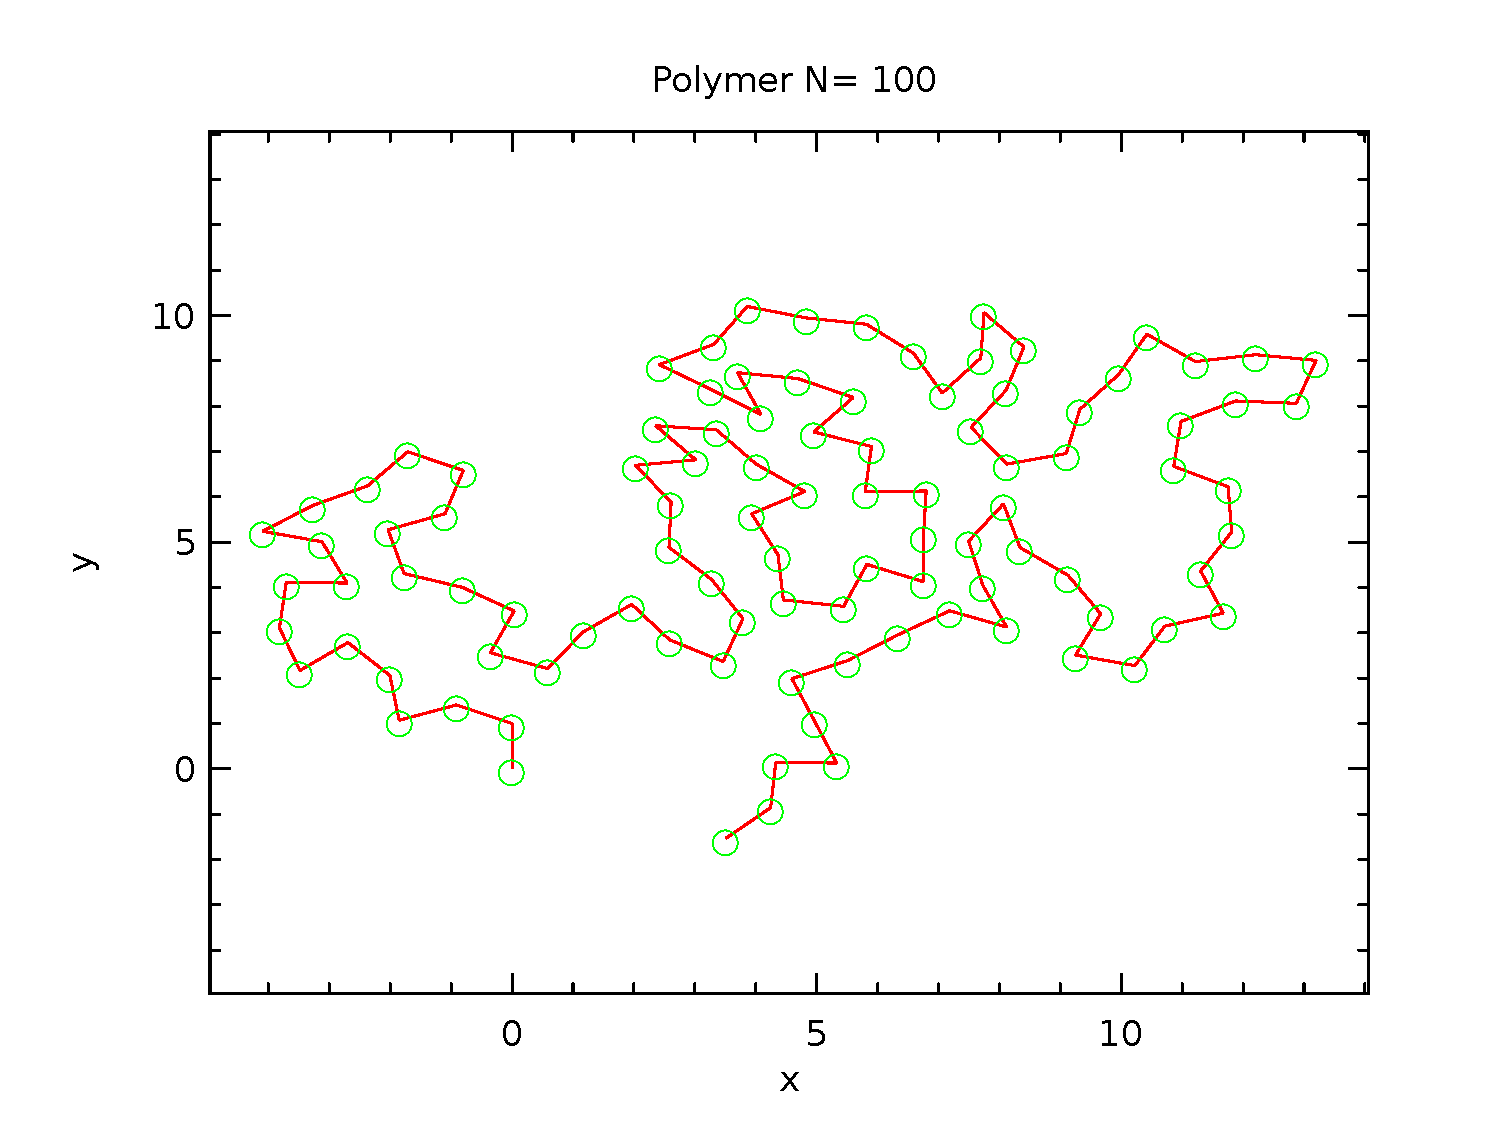
\includegraphics[width=0.5\textwidth]{voorblad.pdf}
\caption{Gyradius $G$ as a function of polymer length $N$. The data is fitted to $G=a\cdot N^b$}
\label{fig:gyradius}
\end{figure}